\section{Setup}
\label{sec:setup}

%% tikz: setup
%\begin{figure}[H]
%	\centering

%	\caption[Simulation Setup]{Simulation Setup: \itshape The microphones (green circles) are placed on a rectangular border around the possible source locations.}
%	\label{fig:setup}
%\end{figure}


% setup (png)
\begin{figure}[H]
	\centering
%	% This file was created by matlab2tikz.
%
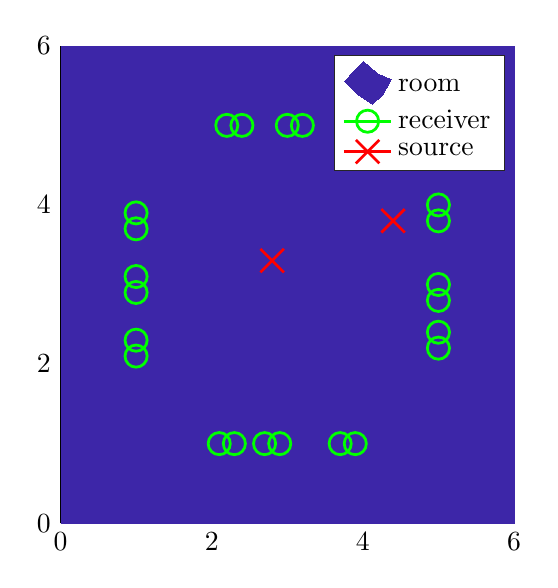
\begin{tikzpicture}

\begin{axis}[%
width=0.475\textwidth,
height=0.5\textwidth,
at={(0\textwidth,0\textwidth)},
scale only axis,
xmin=-0,
xmax=6,
ymin=-0,
ymax=6,
axis background/.style={fill=white},
axis x line*=bottom,
axis y line*=left,
legend style={legend cell align=left, align=left, draw=white!15!black}
]

\addplot[%
surf,
shader=interp, colormap={mymap}{[1pt] rgb(0pt)=(0.239216,0.14902,0.658824); rgb(1pt)=(0.239216,0.14902,0.658824)}, mesh/rows=6]
table[row sep=crcr, point meta=\thisrow{c}] {%
%
x	y	c\\
0	0	0\\
0	1.2	0\\
0	2.4	0\\
0	3.6	0\\
0	4.8	0\\
0	6	0\\
1.2	0	0\\
1.2	1.2	0\\
1.2	2.4	0\\
1.2	3.6	0\\
1.2	4.8	0\\
1.2	6	0\\
2.4	0	0\\
2.4	1.2	0\\
2.4	2.4	0\\
2.4	3.6	0\\
2.4	4.8	0\\
2.4	6	0\\
3.6	0	0\\
3.6	1.2	0\\
3.6	2.4	0\\
3.6	3.6	0\\
3.6	4.8	0\\
3.6	6	0\\
4.8	0	0\\
4.8	1.2	0\\
4.8	2.4	0\\
4.8	3.6	0\\
4.8	4.8	0\\
4.8	6	0\\
6	0	0\\
6	1.2	0\\
6	2.4	0\\
6	3.6	0\\
6	4.8	0\\
6	6	0\\
};
\addlegendentry{room}

\addplot [color=green, line width=1.0pt, draw=none, mark size=4.0pt, mark=o, mark options={solid, green}]
  table[row sep=crcr]{%
2.1	1\\
2.3	1\\
2.7	1\\
2.9	1\\
3.7	1\\
3.9	1\\
5	2.2\\
5	2.4\\
5	2.8\\
5	3\\
5	3.8\\
5	4\\
2.2	5\\
2.4	5\\
3	5\\
3.2	5\\
3.8	5\\
4	5\\
1	2.1\\
1	2.3\\
1	2.9\\
1	3.1\\
1	3.7\\
1	3.9\\
};
\addlegendentry{receiver}

\addplot [color=red, line width=1.0pt, draw=none, mark size=6.0pt, mark=x, mark options={solid, red}]
  table[row sep=crcr]{%
4.4	3.8\\
2.8	3.3\\
};
\addlegendentry{source}

\end{axis}
\end{tikzpicture}% % tikz-data
%   \includegraphics[width=\textwidth]{data/plots/setup/setup.pdf}
	\includegraphics[width=0.8\textwidth]{data/plots/setup/setup.png}
	\caption[Simulation Setup]{Simulation Setup: \itshape The microphones (green circles) are placed on a rectangular border around the possible source locations (white dots). Two example source positions are shown (red crosses).}
	\label{fig:setup}
\end{figure}


The setup, that is going to be simulated, consists of a rectangular room with sides of 6 metres length in all 3 dimensions.\alt{, that is 6m wide, 6m long and 6m high.} Figure \ref{fig:setup} shows the room in blue color from a top-down perspective. Placed in this room, there are a total of 12 microphone pairs, 3 of them on each wall, shown in green. The sources are shown in red. The white dot matrix represents the discrete locations a source can be placed within the room. They also represent the mean of each component of the gaussian mixture model introduced in section \ref{sec:gmm}.

% Reason for the positions of microphones and possible source positions
Originally, the microphones had been placed adjacent to the walls, but first trials have shown that the reflections from the wall decreased localisation performance. Therefore, to be able to evaluate the other parameters independent from the influence a close wall has on the received signal, the microphone pairs have been inset by 10 points (or 1 metre) from the walls. The same decision had to be made in regards to the possible locations a source could be in. First results indicated that localisation performance was significantly impaired, when sources were located in the border area behind the microphones. In order to create reasonable base conditions, the location of the sources was therefore restricted to the inside of the area the microphone pairs enclose. Further examination showed, that the same was true for positions very close to the microphones, which is why the area of possible source locations had to be further decreased by 2 points (or 20 centimetres).

\alt{are going to be placed within this room with fixed or random positions, depending on the evaluation scenario, and are described using one-dimensional position vectors with x-, y- and z-coordinates (i.e. $\begin{bmatrix} 2&3&3  \end{bmatrix}$ describes a source at the position $x=3, y=3$ and $z=3$)}
